\section{Optimizing t-SNE Hyperparameters}

\subsection{Automated Stopping of EE and t-SNE Run}
In this section, we will explain how opt-SNE \cite{belkina19} improves on Barnes-Hut t-SNE. 

\subsection{Informative Initialization}
The standard t-SNE algorithm starts with an initization $y_i^{(0)}$ for $i=\{1, 2, \dots, n\}$ which are drawn independently from $\mathcal{N}(0, \delta^2 I)$ for some small $\delta > 0$, see \cite{vdMaa08} and \cite{vdMaa14}. 

However, recent work \cite{kobak21} has shown that informative initialization leads to embeddings that better preserve large-scale structures within the data. 
They argue that using informative intialization should be the default option for t-SN
E.
Indeed, modern implementations of t-SNE in libraries like openTSNE \cite{openTSNE} or Scikit-learn now all use PCA initialization by default. 
This means that we perform a principal component analysis on the input data $x_1, \dots, x_n$ and use the output $y_1, \dots, y_n$ as the initial points for the low-dimensional embedding. 

%\begin{figure}[h]
  %  \centering 
   % 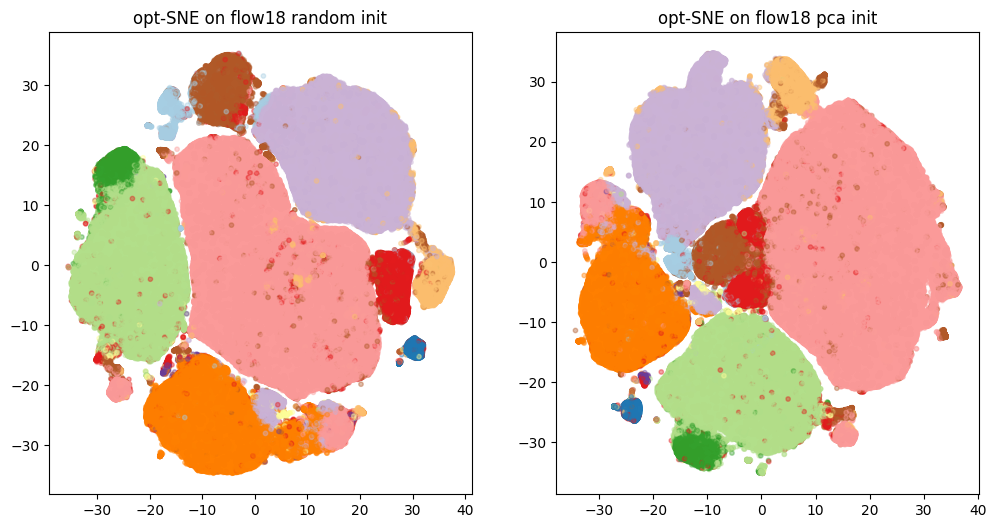
\includegraphics[width=\linewidth]{figures/pca_vs_random_init.png}
   % \caption{PCA versus random initialization}
   % \label{fig:PCA_vs_random}
%\end{figure}
In our experiments, we do not necessarily see a visual improvement of the PCA initialized embedding over the random initialization one, but \textcolor{red}{one should look at other metrics to see how well the global structure is preserved e.g. Pearson correlation or Spearman correlation}. 

\subsection{Current State of Literature of Parameter Choices}
Here, I want to collect guidelines for choosing t-SNE parameters. It could be interesting to look at this from the perspective of a practitioner, using t-SNE libraries like openTSNE or the scikit-learn implementation and investigate if the default choices lead to good results. 

